\documentclass{article}
\usepackage{graphicx} % Required for inserting images

\title{CPE301 Final Report}
\author{Eric Austin and Omar Acebedo Vega}
\date{May 12 2024}

\begin{document}

\maketitle

\section{Introduction}
The goal of this final lab was to create an evaporation cooling system(swamp cooler). The purpose was to build a working cooler using the Arduino
2560 and sensors from the Arduino kit. We are to use all knowledge from all previous labs to complete the swamp cooler.
\section{Procedure}
For this lab, we set up a water cooler using an Arduino and a breadboard. We were instructed not to use certain Arduino library functions like pinMode, digitalRead, digitalWrite, delay, analogRead, and Serial(). Our circuit operates through four states: Disabled, Idle, Running, and Error, performing specific tasks in each.

Initially, the circuit is in the Disabled state, where the LCD shows "system is ready," the yellow LED and stepper motor are active, and they remain so until the start button is pressed. Pressing the start button changes the state to Idle. In this state, a green LED lights up, and the LCD displays the current temperature and humidity while the stepper motor continues to move. The green LED indicates that the sensor has detected water in the container.

If the stop button is pressed, the circuit returns to the Disabled state and starts over. If the water level falls below a set threshold, the circuit enters the Error state, indicated by a red LED, with the LCD displaying "Water level is too low," and the motor turning off. In this state, pressing the restart button switches back to Idle, or pressing the stop button returns to Disabled.

In the Running state, the fan motor operates, the LCD shows the current temperature and humidity, the stepper motor rotates, and a blue LED lights up. The circuit transitions from Running to Error if the water level is too low, or to Idle if the temperature falls below the threshold. Pressing the stop button at any time in Running will switch back to Disabled. Any changes will continue through the cycle as outlined in the diagram.








\section{Result}
The Arduino Mega 2560 board connects and powers most components of our project. We use the Arduino IDE to program this board to manage the system’s temperature and humidity.

The system uses four LEDs to indicate different states: Yellow for Disabled, Green for Idle, Blue for Running, and Red for Error. In the Disabled state, activated by the yellow LED, the system powers on but all components remain off. This state can also be entered by pressing the stop button from any state. The Green LED indicates the Idle state, triggered by the start button from the Disabled state, where the system begins to monitor temperature and humidity continuously.

The system moves between the Running and Idle states based on temperature comparisons with a set threshold. It enters the Running state, shown by the Blue LED, when the temperature exceeds the threshold, turning the fan on. It switches to the Idle state if the temperature falls below the threshold.

Water levels control the transition between the Idle and Error states. If the water level is at or below a certain threshold, the system enters the Error state, indicated by the Red LED, signaling low water with a potential to stop the system. Pressing the reset button can return the system to Idle if the water is above the critical level.


\section{Links}
Github repository: https://github.com/EricPAustin/CPE301-Final-Project


\begin{figure}
\centering
\includegraphics[width=0.5\textwidth]{IMG_2056.jpg}
\caption{\label{fig:img1}Above is a picture of our cooler circuit}
\end{figure}

\begin{figure}
\centering
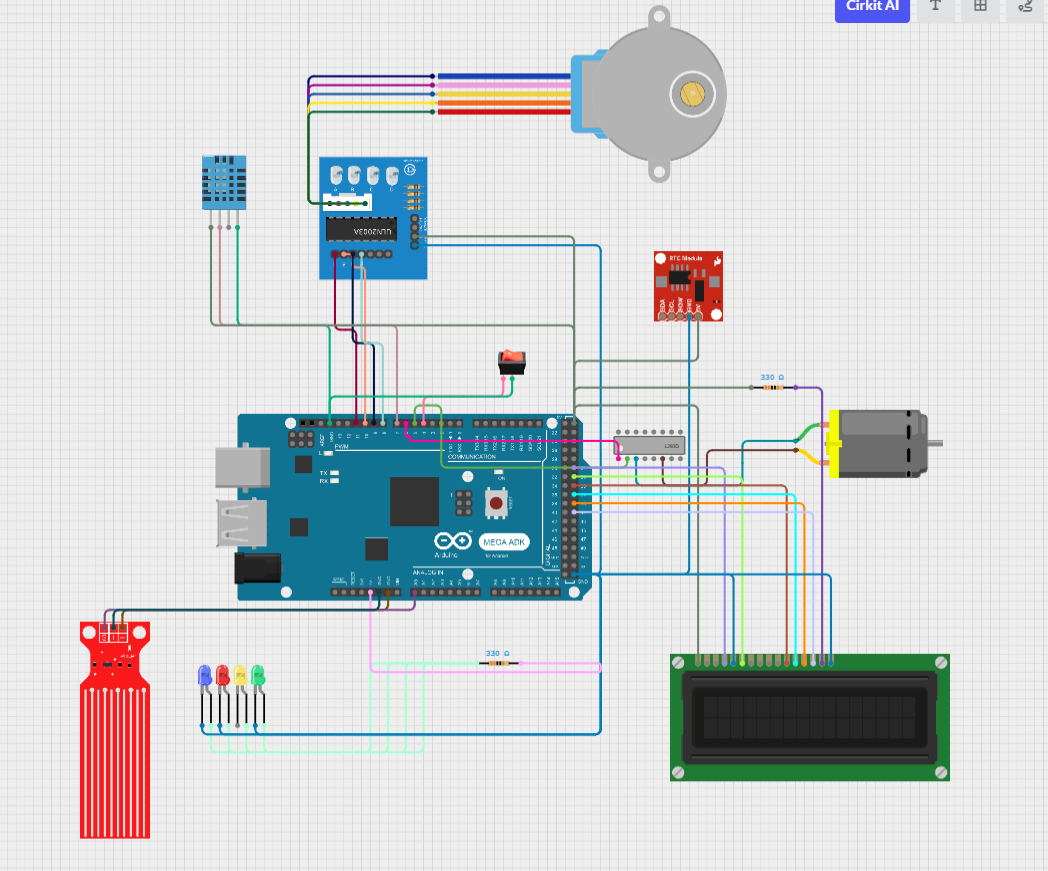
\includegraphics[width=0.5\textwidth]{image.png}
\caption{\label{fig:img2}Above is our schematic}
\end{figure}
    


\end{document}
